Before a flight trajectory can be computed, all the forces acting on the vehicle must
be known. On an airplane or rocket, the primary forces are lift, drag, thrust, and
weight as shown in \cref{fig:forces-acting-on-vehicle}. Lift and drag forces are
aligned with the wind-axis system, thrust forces are aligned relative to the body-axis
system, and weight forces are aligned with the gravity vector.

\begin{figure}[htbp]
  \centering
  \begin{tikzpicture}[scale=0.92,>=Latex,line cap=round,line join=round]
  % Stylized vehicle outline, redrawn from the source figure.
  \draw[line width=0.9pt]
    (-3.2,0.55) .. controls (-2.35,0.50) and (-1.55,0.32) .. (-0.70,0.08)
    -- (0.70,-0.28) .. controls (1.15,-0.40) and (1.45,-0.32) .. (1.62,-0.08)
    .. controls (1.74,0.10) and (1.65,0.28) .. (1.38,0.36)
    -- (0.55,0.62) -- (0.10,1.10) -- (-0.72,0.88)
    -- (-1.15,0.45) -- (-2.45,0.78) -- cycle;
  \draw[line width=0.9pt] (-3.2,0.55) .. controls (-2.45,0.78) and (-1.75,0.65) .. (-0.90,0.30);
  \draw[line width=0.9pt] (-1.15,0.45) -- (-0.45,-0.22) -- (0.25,-0.38) -- (0.72,-0.28);
  \draw[line width=0.9pt] (1.38,0.36) -- (1.28,0.92) -- (0.72,1.18) -- (0.10,1.10);
  \draw[line width=0.9pt] (1.42,0.30) ellipse [x radius=0.18,y radius=0.34];

  \draw[->,line width=0.9pt] (-3.05,0.57) -- (-4.25,0.92)
    node[left] {Thrust};
  \draw[->,line width=0.9pt] (-0.15,0.55) -- (-0.05,1.95)
    node[above] {Lift};
  \draw[->,line width=0.9pt] (-0.20,-0.05) -- (-0.20,-1.30)
    node[below] {Weight};
  \draw[->,line width=0.9pt] (1.55,-0.02) -- (2.95,-0.55)
    node[right] {Drag};
\end{tikzpicture}

  \caption{Forces acting on vehicle.}
  \label{fig:forces-acting-on-vehicle}
\end{figure}

Lift and drag forces are normally given in terms of nondimensional lift and drag
coefficients and a reference area. These aerodynamic coefficients are difficult to
predict; they are often computed with aerodynamic-prediction software, such as
Missile Datcom\taosref{18} and Sandiac\taosref{19}, or they are obtained from wind
tunnel tests. The result is a tabulated set of aerodynamic coefficients that is often a
function of Mach number, altitude, and angle of attack. For example,
\cref{fig:axial-force-mach} shows the axial-force coefficient as a function of Mach
number.

\begin{figure}[htbp]
  \centering
  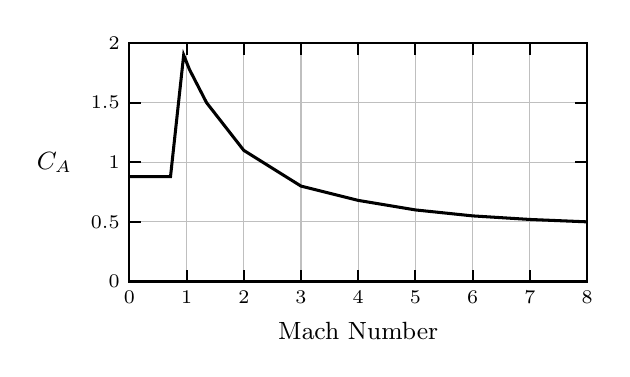
\begin{tikzpicture}
\begin{axis}[
  width=0.61\linewidth,
  height=0.38\linewidth,
  xmin=0,xmax=8,
  ymin=0,ymax=2,
  xtick={0,1,...,8},
  ytick={0,0.5,1,1.5,2},
  grid=major,
  axis line style={line width=0.8pt},
  tick style={black,line width=0.7pt},
  xlabel={Mach Number},
  ylabel={$C_A$},
  ylabel style={rotate=-90},
  label style={font=\small},
  tick label style={font=\scriptsize}
]
\addplot[black,line width=1.1pt] coordinates {
  (0,0.88) (0.72,0.88) (0.95,1.90) (1.05,1.78) (1.35,1.50)
  (2,1.10) (3,0.80) (4,0.68) (5,0.60) (6,0.55) (7,0.52) (8,0.50)
};
\end{axis}
\end{tikzpicture}

  \caption{Axial force coefficient as a function of Mach number.}
  \label{fig:axial-force-mach}
\end{figure}

Thrust and mass-flow data for jet and rocket motors are usually obtained from
analysis software or from tests. Again, this data is normally tabulated because no
analytical functions exist. For jet engines, thrust and fuel flow are typically a
function of Mach number, altitude, and power setting. For rocket motors, thrust and
mass flow are usually given as functions of time, as shown in
\cref{fig:thrust-mass-flow-time}.

\begin{figure}[htbp]
  \centering
  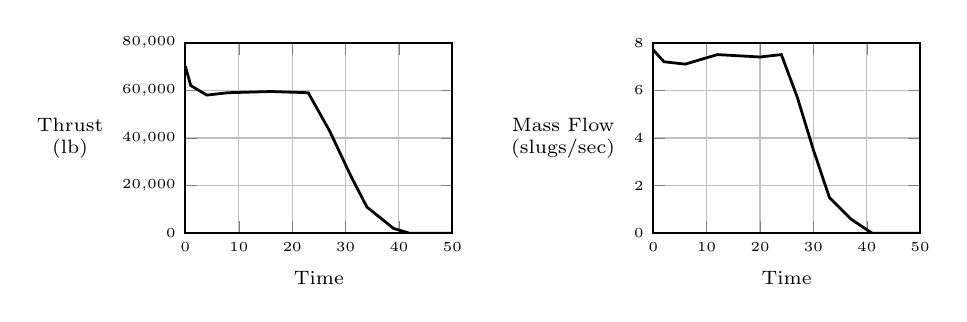
\begin{tikzpicture}
\begin{axis}[
  at={(0cm,0cm)},anchor=south west,
  width=0.41\linewidth,height=0.33\linewidth,
  xmin=0,xmax=50,ymin=0,ymax=80000,
  xtick={0,10,...,50},ytick={0,20000,...,80000},
  scaled y ticks=false,
  grid=major,
  xlabel={Time},ylabel={Thrust\\(lb)},
  ylabel style={align=center,rotate=-90},
  label style={font=\scriptsize},tick label style={font=\tiny},
  axis line style={line width=0.7pt}
]
\addplot[black,line width=1.0pt] coordinates {
  (0,70000) (1,62000) (4,58000) (8,59000) (16,59500) (23,59000)
  (27,43000) (31,24000) (34,11000) (39,2000) (42,0) (50,0)
};
\end{axis}
\begin{axis}[
  at={(0.49\linewidth,0cm)},anchor=south west,
  width=0.41\linewidth,height=0.33\linewidth,
  xmin=0,xmax=50,ymin=0,ymax=8,
  xtick={0,10,...,50},ytick={0,2,...,8},
  grid=major,
  xlabel={Time},ylabel={Mass Flow\\(slugs/sec)},
  ylabel style={align=center,rotate=-90},
  label style={font=\scriptsize},tick label style={font=\tiny},
  axis line style={line width=0.7pt}
]
\addplot[black,line width=1.0pt] coordinates {
  (0,7.7) (2,7.2) (6,7.1) (12,7.5) (20,7.4) (24,7.5)
  (27,5.7) (30,3.5) (33,1.5) (37,0.6) (41,0) (50,0)
};
\end{axis}
\end{tikzpicture}

  \caption{Thrust and mass flow as a function of time.}
  \label{fig:thrust-mass-flow-time}
\end{figure}

Tabulated data defining forces on the vehicle are input to TAOS with table files.
Each table file consists of one or more tables, with each table identified by a name,
as shown in \cref{fig:table-files-and-tables}. A table defines a single value, such as
thrust or mass flow. This value can be a constant, it can be interpolated from
tabulated data, it can be computed from an equation, or it can be computed from a
combination of interpolations and equations.

\begin{figure}[htbp]
  \centering
  \begin{tikzpicture}[>=Latex,font=\small]
  \coordinate (boxsw) at (0,0);
  \draw[line width=0.9pt] (0,0) -- (0,5.25) -- (4.0,5.25) -- (4.0,0.35)
    .. controls (3.65,0.15) and (3.35,0.15) .. (3.00,0.35)
    .. controls (2.65,0.55) and (2.35,0.55) .. (2.00,0.35)
    .. controls (1.65,0.15) and (1.35,0.15) .. (1.00,0.35)
    .. controls (0.65,0.55) and (0.35,0.55) .. (0,0.35) -- cycle;
  \draw[line width=0.9pt] (0,3.45) -- (4.0,3.45);
  \draw[line width=0.9pt] (0,1.80) -- (4.0,1.80);

  \node[anchor=north west,font=\ttfamily] at (0.15,5.10) {(table-1)};
  \node[align=center] at (2.0,4.15) {Data defining a\\thrust value};
  \node[anchor=north west,font=\ttfamily] at (0.15,3.32) {(table-2)};
  \node[align=center] at (2.0,2.55) {Data defining a\\mass flow value};
  \node[anchor=north west,font=\ttfamily] at (0.15,1.68) {(table-3)};
  \node at (2.0,1.05) {etc.};

  \node[align=center] (names) at (-2.0,3.10) {Table\\names};
  \draw[->,line width=0.8pt] (names.east) -- (0,4.92);
  \draw[->,line width=0.8pt] (names.east) -- (0,3.20);
  \draw[->,line width=0.8pt] (names.east) -- (0,1.55);

  \draw[decorate,decoration={brace,amplitude=7pt},line width=0.8pt]
    (4.45,5.20) -- (4.45,0.35);
  \node[align=left,anchor=west] at (4.85,2.80)
    {Table file contains\\one or more tables};
\end{tikzpicture}

  \caption{Table files and tables.}
  \label{fig:table-files-and-tables}
\end{figure}
